% !TEX root = ../../book.tex

\chapter{Advanced Topics}


In this chapter we want to discuss some advanced methods that are applicable in the context of trading. This chapter is broadly divided into two main areas; the first covers topics which are extensions of models discussed in Chapter 2 in the low frequency context. Although the state-space modeling is discussed in the context of ARIMA, its scope is much wider. We also outline the established methodology for studying regime switching, but indicate the areas of further research where predicting ahead when the regime shift is likely to occur using signals form the past is of great interest. This is followed by a discussion on using volume information to study the price volatility. With the increased exploitation of price behavior data, it has become necessary to look for additional signals. We present a theoretical model that shows that there is correlation between volume traded and volatility when there is information flow. The second area of this chapter focuses on the models from point processes to study the higher frequency data. Here our approach has been to provide an intuitive discussion of main tools; as readers will realize, the trade data is quite noisy and there is a great deal of scope to do research especially in non-parametric modeling of arrivals and cancellations in the limit order market. 


\section{State-Space Modeling} 


There has been much recent interest in the representation of ARIMA models in the state-space form, for purpose of forecasting, as well as for model specification and maximum likelihood estimation of parameters. This approach helps to update the model coefficients as and when new data arrives. 


The state-space models were initially developed by control systems engineers to measure a signal contaminated by noise. The signal at time ``$t$'' is taken to be a linear combination of variables, called state variables that form the so called state vector at time, $t$. The key property of the state vector is that it contains the minimum set of information from past and present data but the future behavior of the system is independent of the past value and depends only on the present values. Thus the state vector evolves according to the Markov property. The state equation is stated as,
	\begin{equation}\label{eqn:2zt}
	Z_t = \Phi_tZ_{t-1} + a_t
	\end{equation}
and observation equation
	\begin{equation}\label{eqn:2yt}
	Y_t = H_tZ_t + N_t
	\end{equation}
where it is assumed that $a_t$ and $N_t$ are independent white-noise processes; $a_t$ is a vector white noise with covariance matrix $\Sigma_a$ and $N_t$ has variance $\sigma_N^2$. The matrix $\Phi_t$ in (\ref{eqn:2zt}) is an $r \times r$ transition matrix and $H_t$ in (\ref{eqn:2yt}) is a $l \times r$ vector, which are allowed to vary in time.


We will consider the state-space form of an ARIMA$(p,d,q)$ process $\phi(B)Y_t = \theta(B)\,\varepsilon_t$, define the forecasts $\hat{Y}_t(j) = E(Y_{i+j}\,|\,Y_t,Y_{t-1},...)$ for $j= 0,1,\ldots,r$, with $r= \max(p+d,q+1)$, and $\hat{Y}_t(0) = Y_t$.


From the updating equations $\hat{Y}_{t+1}(l) = \hat{Y}_t(l+1) + \psi_l\varepsilon_{t+1}= \hat{Y}_t(l + 1) + \psi_l\, [Y_{t+1} - \hat{Y}_t(1)]$ for the general ARIMA model, we have that $\hat{Y}_t(j - 1)= \hat{Y}_{t-1}(j) + \psi_{j-1}\varepsilon_t$, $j = 1,2,\ldots,r-1$. Also for $j= r>q$, observe that $\hat{Y}_t(j-1)= \hat{Y}_{t-1}(j) + \psi_{j-1}\varepsilon_t = \sum_{i=1}^{p+d}\phi_i\hat{Y}_{t-1}(j - i) + \psi_{j-1}\varepsilon_t$. So we define the ``state'' vector at time $t$, $Z_t$, with $r$ components as $Z_t = (Y_t, \hat{Y}_t(1),\cdots,\hat{Y}_t(r-1))'$. Then from the above relations we find that $Z_t$ satisfies the equations
	\[ 
	Z_t = \begin{bmatrix}
                        0 & 1 & 0 & \cdots & 0 \\
                        0 & 0 & 1 & \cdots &  0 \\
                        \vdots & \vdots &\ddots  &  &  \vdots \\
                        0 & 0 &  & \ddots &  1 \\
                        \phi_r & \phi_{r-1} & \cdots & \cdots &  \phi_1
                    \end{bmatrix}
                    \,Z_{t-1} + 
                    \begin{bmatrix}
                    1\\ \vdots \\ \vdots \\ \psi_{r-1}
                    \end{bmatrix}
                    \,\varepsilon_t
                    \]
where $\phi_i = 0$ if $i > p + d$. So we have
	\begin{equation}\label{eqn:2secondzt}
	Z_t = \Phi Z_{t-1} + \Psi\varepsilon_t
	\end{equation}
together with the observation equation
	\begin{equation}\label{eqn:2thirdzt}
	Z_t = Y_t + N_t = [1,0,\ldots,0] \,Z_t + N_t = H Z_t + N_t
	\end{equation}
where the additional noise $N_t$ would be present only if the ARIMA process $\{Y_t\}$ is observed subject to additional noise; otherwise we simply have $Z_t \equiv Y_t = HZ_t$. The above two equations constitute what is known as a state-space representation of the ARIMA model. We note that there are many other constructions of the state vector $Z_t$ that will give rise to state-space equations of the general form of (\ref{eqn:2zt})--(\ref{eqn:2yt}); that is, the state-space form of an ARIMA model is not unique.

Observe, in applications the matrices $\Phi_t$ and $H_t$ are constant matrices, $\Phi \equiv \Phi_t$ and $H \equiv H_t$ for all $t$, that do not depend on $t$, as in the state-space form (\ref{eqn:2secondzt})--(\ref{eqn:2thirdzt}) of the ARIMA model. In this case the system or model is said to be time-invariant. A nice feature of expressing a model in state-space form is that an updating procedure can be readily used when a new observation becomes available to revise the current state vector and to produce forecasts. These forecasts in general tend to fare better. 

For the state-space model, define the finite sample estimates of the state vector $Z_{t+1}$ based on observations $Y_t,\cdots,Y_l$ over the finite past time period, as
	\[
	\hat{Z}_{t+l|t} = E[Z_{t+l}|Y_t,\cdots,Y_l],\text{ with } V_{t+l|t} = E[(Z_{t+l} - \hat{Z}_{t+l|t})(Z_{t+l} - \hat{Z}_{t+l|t})'].
	\]
A convenient computational procedure, known as the \textit{Kalman filter equations}, is then available to obtain the current estimate $\hat{Z}_{t|t}$, in particular. It is known that, starting from some appropriate initial values $Z_0 \equiv \hat{Z}_{0|0}$ and $V_0 \equiv V_{0|0}$, the optimal filtered estimate, $\hat{Z}_{t|t}$, is given through the following recursive relations:
	\begin{equation}\label{eqn:2hatz}
	\hat{Z}_{t|t} = \hat{Z}_{t|t-1} + K_t(Y_t - H_t\hat{Z}_{t|t-1})
	\end{equation}
where $K_t= V_{t|t-1} H_t'[H_t V_{t|t-1} H_t' + \sigma_N^2]^{-1}$ with $\hat{Z}_{t|t-1} = \Phi_t \hat{Z}_{t-1|t-1},V_{t|t-1} = \Phi_t V_{t-1|t-1} \Phi_t' + \Sigma_{a}$ and $V_{t|t} = [I - K_tH_t] V_{t|t-1} = V_{t|t-1} - V_{t|t-1} H_t' [H_t V_{t|t-1} H_t' + \sigma_N^2]^{-1} H_t V_{t|t-1}$ for $t=1,2,\cdots$.


In (\ref{eqn:2yt}), the quantity $\varepsilon_{t|t-1}= Y_t - H_t \hat{Z}_{t|t-1} \equiv Y_t - \hat{Y}_{t|t-1}$ is called the (finite sample) innovation at time $t$, because it is the new information provided by the measurement $Y_t$ which was not available from the previous observed (finite) history of the system. The factor $K_t$ is called the ``Kalman gain'' matrix. The filtering procedure in (\ref{eqn:2hatz}) has the recursive ``prediction-correction'' or ``updating'' form, and the validity of these equations as representing the minimum mean square error predictor can readily be verified through the principles of ``updating''. For example, verification of (\ref{eqn:2hatz}) follows from the principle, for linear prediction, that
	\[
	\begin{split}
	E[Z_t\,|\,Y_t,\ldots,Y_1]&= E[Z_t|Y_t - \hat{Y}_{t|t-1},Y_{t-1},\cdots,Y_1] \\
	&= E[Z_t\,|\,Y_{t-1},\cdots,Y_1] + E[Z_t \,|\, Y_t - \hat{Y}_{t|t-1}],
	\end{split}
	\]
since $\varepsilon_{t|t-1} = Y_t - \hat{Y}_{t|t-1}$ is independent of $Y_{t-1},\ldots,Y_1$. From (\ref{eqn:2hatz}) it is seen that the estimate of $Z_t$ based on observations through time $t$ equals the prediction of $Z_t$ from observations through time $t-1$ updated by the factor $K_t$ times the innovation $\varepsilon_{t|t-1}$. The quantity $K_t$ can be interpreted as the regression coefficients of $Z_t$ on the innovation $\varepsilon_{t|t-1}$, with $\Var(\varepsilon_{t|t-1}) = H_t V_{t|t-1} H_t' + \sigma_N^2$ and $\Cov(Z_t,\varepsilon_{t|t-1})= V_{t|t-1}H_t'$ following directly from (\ref{eqn:2thirdzt}) since $\varepsilon_{t|t-1} = H_t (Z_t - \hat{Z}_{t|t-1}) + N_t$. Thus, the general \textit{updating relation} is $\hat{Z}_{t|t} = \hat{Z}_{t|t-1} + \Cov(Z_t,\varepsilon_{t|t-1})\{\Var(\varepsilon_{t|t-1})\}^{-1}\varepsilon_{t|t-1}$, where $\varepsilon_{t|t-1} = Y_t - \hat{Y}_{t|t-1}$, and the relation in $V_t$ is the usual updating of the error covariance matrix to account for the new information available from the innovation $\varepsilon_{t|t-1}$, while the \textit{prediction relations} (\ref{eqn:2hatz}) follow directly from (\ref{eqn:2secondzt}). In general, forecasts of future state values are available directly as $\hat{Z}_{t+l|t} = \Phi_{t+l} \hat{Z}_{t+l-1|t}$ for $l = 1,2,\ldots$ with the covariance matrix of the forecast errors generated recursively essentially through (\ref{eqn:2pteq}) as $V_{t+l|t} = \Phi_{t+l}V_{t+l-1|t} \Phi_{t+l}' + \Sigma_a$. Finally, forecasts of future observations $Y_{t+l}$ are then available as $\hat{Y}_{t+l|t} = H_{t+l} \hat{Z}_{t+l|t}$, since $Y_{t+l|t} = H_{t+l} Z_{t+l} + N_{t+l}$, with forecast error variance $v_{t+l|t} = E[(Y_{t+l} - \hat{Y}_{t+l|t})^2] = H_{t+l}V_{t+l|t}H_{t+l}' + \sigma_N^2$.


For ARIMA models, with state-space representation (\ref{eqn:2secondzt})--(\ref{eqn:2thirdzt}) and $Y_t = HZ_t$ with $H = [1,0,\ldots,0]$, this Kalman filtering procedure constitutes an alternate method to obtain exact finite sample forecasts, based on data $Y_t,Y_{t-1},\cdots,Y_1$, for future values in the ARIMA process, subject to specification of appropriate initial conditions to use in the terms in (\ref{eqn:2hatz}). For stationary zero-mean processes $Y_t$, the appropriate initial values are $\hat{Z}_{0|0} = 0$, a vector of zeros, and $V_{0|0} = \Cov(Z_0) \equiv V_*$, the covariance matrix of $Z_0$ which can easily be determined under stationarity through the definition of $Z_t$. Specifically, since the state vector $Z_t$ then follows the stationary vector AR(1) model $Z_t = \Phi Z_{t-1} + \psi\varepsilon_t$, its covariance matrix $V_*= \Cov(Z_t)$ satisfies $V_*= \Phi V_*\Phi' + \sigma_{\varepsilon}^2\Psi\Psi'$, which can be readily solved for $V_*$. For nonstationary ARIMA processes, additional assumptions need to be specified. The ``steady-state'' values of the Kalman filtering procedure $l$-step ahead forecasts $\hat{Y}_{t+l|t}$ and their forecast error variances $v_{t+l|t}$, which are rapidly approached as $t$ increases, will be identical to the expressions given previously, $\hat{Y}_t(l)$ and $\sigma^2(l) = \sigma^2(1 + \sum_{i=1}^{i-1}\psi_{i}^2)$


In particular, for the ARIMA process in state-space form, we can obtain the exact (finite sample) one-step ahead forecasts $\hat{Y}_{t-1}(1) = E[Y_t\,|\,Y_{t-1},\ldots,Y_1] = H \hat{Z}_{t|t-1}$, and their error variances $v_{t|t-1} = H V_{t|t-1} H'$, conveniently through the Kalman filtering equation (\ref{eqn:2hatz}). This can be particularly useful for evaluation of the Gaussian likelihood function, based on $T$ observations $Y_1,\cdots,Y_T$ from the ARIMA process, applied to the problem of maximum likelihood estimation of model parameters.

This state-space approach to exact likelihood function determination has also been shown to be quite useful in dealing with estimation problems for ARMA models when some values $Y_t$ of the series are not observed, that is, there are missing values among the sequence of $Y_t$ values.

An alternative set-up, alternative to (\ref{eqn:2thirdzt}) and (\ref{eqn:2hatz}) is to assume that the deviations in the observation and transition equations are related. With the observation equation stated in (\ref{eqn:2yt}), the transition equation is modified as 
	\begin{equation}\label{eqn:223zt}
	Z_t = \Phi Z_{t-1} + \alpha N_t 
	\end{equation}
This model studied in Ord, Koehler, and Snyder (1997)~\cite{ord1997estimation} with a single source of error $(N_t)$ is shown to be closely related to various exponential smoothing procedures. There are other formulations of state-space models, such as structural models by Harvey (1989)~\cite{harvey1989kalman} and dynamic linear models of West and Harrison (1997)~\cite{west1997} that are found to be useful for model building.


We provide two examples to illustrate the application of the models (\ref{eqn:2secondzt}) and (\ref{eqn:2thirdzt}) in the broader context of this book. The slope in a local linear trend is a random walk. Specifically,
	\begin{equation}\label{eqn:randomwalk}
	\begin{split}
	p_t&= \mu_t+ e_t \\
	\mu_t&= \mu_{t-1} + \delta_{t-1} + \eta_{0t} \\
	\delta_t&=\delta_{t-1}+\eta_{1t}
	\end{split}
	\end{equation}
Here the trend is composed of level `$\mu_t$' and slope `$\delta_t$'. The slope `$\delta_t$' when written as 
	\begin{equation}\label{eqn:slopewritten}
	\delta_t= D+ e(\delta_{t-1} - D)+ \eta_{1t}
	\end{equation}
in AR(1) form is sometimes known as generalized local linear trend. These models can be written in the form of (\ref{eqn:2secondzt}) and (\ref{eqn:2thirdzt}); the updating process given in (\ref{eqn:2hatz}) can be used to accommodate a wide range of models.


Menkveld, Koopman and Lucas (2007)~\cite{menkkoop} study the price discovery process for stocks that are cross-listed in two different markets via state-space models. The question if the trading location matters more than business location is of intent to finance researchers. Consider a stock traded in Amsterdam and in NY exchanges. Because of the time difference, there is only an hour of overlap in trading. Ignoring this aspect, write the two-dimensional price vector as
	\begin{equation}
	\begin{split}
	p_t&=\mu_t + e_T \\
	&=\mu_t + \theta(\mu_t-\mu_{t-1}) + e_t
	\end{split}
	\end{equation}
as the observational equation and the state equation is
	\begin{equation}
	\mu_t= \mu_{t-1} + \xi_t
	\end{equation}
The above can be written in the form of (\ref{eqn:2secondzt}) and (\ref{eqn:2thirdzt}) with appropriate choice of `$\Phi$' and `$H$' matrices. The main advantage of state-space models is that they accommodate the possibility of slowly varying parameters over time, which is more realistic in modeling the real world data. 


\section{Regime Switching and Change-Point Models}


It has been long noted in finance that there are two kinds of recurrences in stock prices: underreaction and overreaction to a series of good or bad news. The securities that have a good record for an extended period tend to become overpriced and have low returns subsequently. Barberis, Shleifer and Vishny (1998)~\cite{vishny} present a model where investor believes that the returns can arise from one of two regimes although returns follow random walk: mean-reverting or trending. The transition probabilities are taken to be fixed and the regime is more likely to stay the same rather than to switch. But the investor's beliefs are updated as and when the returns data are observed. It is presumed that in many instances, we may not discern these shifts directly whether or when they occur but instead can draw probabilistic inference based on the observed behavior posthumously. Hamilton (2016)~\cite{jdham} reviews models for regime-switching applied in several contexts in macroeconomics, building upon the elegant model introduced in Hamilton (1989)~\cite{89ham}. Here in this section, we will cover only studies that are relevant to finance applications, particularly relevant to trading that exploit anomalies. 


Consider the model,
	\begin{equation}\label{eqn:modelham}
	y_t = \mu_{s_t} + \epsilon_t, \quad s_t=1,2
	\end{equation} 
where $y_t$ is the observed variable, such as asset return and $s_t$ represents two distinct regimes and $\epsilon_t$'s are i.i.d.$\sim N(0,\sigma^2)$. Let $\{F_{t-1}\}$ be the information set available as of `$t-1$'. The transition between the regimes is taken to be Markovian,
	\begin{equation}\label{eqn:markprob}
	\text{Prob}(s_t=j \;|\; s_{t-1}=i, F_{t-1})= p_{ij}, \quad i,j=1,2
	\end{equation}
thus leading to an AR(1) model for $\mu_{s_t}$ as
	\begin{equation}\label{eqn:must}
	\mu_{s_t} = \phi_0 + \phi_1 \mu_{s_{t-1}} + a_t
	\end{equation}
where $a_t$ by definition can take four possible values depending upon $s_t$ and $s_{t-1}$. Here $\phi_0=p_{21}\mu_1 + p_{12} \mu_2$ and $\phi_1=p_{11}-p_{21}$. Note the model for $y_t$ in (\ref{eqn:modelham}) is the sum of an AR(1) process and white noise, then from Theorem~\ref{thm:agg}, $y_t \sim$ ARMA(1,1); but because of discrete nature of `$a_t$', (\ref{eqn:modelham}) is a non-linear process. Note that the unknown parameters are $(\mu_1,\mu_2,\sigma,p_{11},p_{22})'=\lambda$ and they can be estimated via maximum likelihood as follows: note $y_t|(s_t=j,F_{t-1})\sim N(\mu_j,\sigma^2)$. The predictive density of $y_t$ is given as,
	\begin{equation}\label{eqn:predden}
	f(y_t \;|\; F_{t-1})= \sum_{i=1}^2 \text{Prob}(s_t=i \;|\; F_{t-1}) \, f(y_t \;|\; s_t=i, F_{t-1})
	\end{equation}
and estimate of $\lambda$ is obtained by maximizing the likelihood function $L(\lambda)=\sum_{t=1}^T \log f(y_t \;|\; F_{t-1}, \lambda)$. Two useful quantities are: \\


\noindent Predicted regime: 
	\begin{equation}\label{eqn:predreg}
	\text{Prob}(s_t=j \;|\; F_{t-1})= p_{1j} \text{Prob}(s_{t-1}=1 \;|\; F_{t-1}) + p_{2j} \,\text{Prob}(s_{t-1}=2 \;|\; F_{t-1})
	\end{equation}
\noindent Optimal forecast:
	\begin{equation}\label{eqn:optfore}
	E(y_t \;|\; F_{t-1})= \sum_{i=1}^2 (\phi_0+\phi_1 \mu_i) \text{Prob}(s_{t-1}=i \;|\; F_{t-1}).
	\end{equation}
The forecast for `$k$' period ahead can be stated as:
	\begin{equation}\label{eqn:period}
	E(y_{t+k} \;|\; F_{t-1}) = \mu+\phi_1^k \sum_{i=1}^2 (\mu_i-\mu)\, \text{Prob}(s_t=i \;|\; F_{t-1})
	\end{equation}
where $\mu=\phi_0/(1-\phi_1)$.


The basic model has been extended to cover multiple regimes and to vector processes. Interested readers should refer to Hamilton (2016)~\cite{jdham} and references therein. Ang and Timmermann (2012)~\cite{timmerman} discuss a model that accounts for changes not only in the mean but also in variances and autocorrelations:
	\begin{equation}\label{eqn:varautoy}
	y_t= \mu_{s_t} + \phi_{s_t} y_{t-1} + \epsilon_t
	\end{equation}
where $\epsilon_t$'s are independent $\sim N(0,\sigma_{s_t}^2)$. Using the data on excess S\&P500 returns, FX returns, etc., it is identified that there are volatility regimes, but no level shifts.


Hamilton (1990)~\cite{90ham} proposes using EM (Expectation-Maximization) algorithm (Dempster, Laird and Rubin (1977)~\cite{dempster}) to obtain the maximum likelihood estimate, instead of recursive filter approach (see Hamilton (1989)~\cite{89ham} to optimize the loglihood of (\ref{eqn:predden}), updated with $y_t$. Note by Bayes' Theorem
	\begin{equation}\label{eqn:bayes}
	\text{Prob}(s_t=j \;|\; F_t) = \dfrac{\text{Prob}(s_t=j \;|\; F_{t-1}) \, f(y_t\;|\; s_t=j, F_{t-1})}{f(y_t \;|\; F_{t-1})}
	\end{equation}
To get an estimate of $p_{ij}$ in step `$l+1$', use 
	\begin{equation}\label{eqn:hatpijl}
	\hat{p}_{ij}^{(l+1)}= \dfrac{\sum_{t=1}^{T-1} \text{Prob}(s_t=i, s_{t+1}=j \;|\; F_t, \hat{\lambda}^{(l)})}{\sum_{t=1}^{T-1} \text{Prob}(s_t=i \;|\; F_t, \hat{\lambda}^{(l)})}
	\end{equation}
and with these estimates obtain the ML estimates of the rest of the parameters ($\mu_1$, $\mu_2$, and $\sigma$) by maximizing the likelihood function. More details can be found in Hamilton (1990)~\cite{90ham}.


There is a vast literature on Bayesian approach to this problem, see for example, Chib (1998)~\cite{chib} and subsequent publications that followed. An interesting application is given in Pastor and Stambaugh (2001)~\cite{pastor}. Lai and Xing (2013)~\cite{laixing} study a general model, somewhat similar to (\ref{eqn:varautoy}):
	\begin{equation}\label{eqn:arxgarch}
	\text{ARX-GARCH:} \quad y_t= \beta_t' x_t + v_t \sqrt{h_t} \, \epsilon_t
	\end{equation}
where $h_t\sim$ GARCH$(p,q)$ and $\beta_t$ and $v_t$ are piecewise linear. Using the weakly returns of S\&P500 index, AR(1)-GARCH(1,1) model is attempted and it is identified that 1998--2003 had higher volatility. Figure~\ref{fig:sp500} provides the plot of closing price, returns, volatility and volume data. 


	\begin{figure}[!ht]
	\centering
	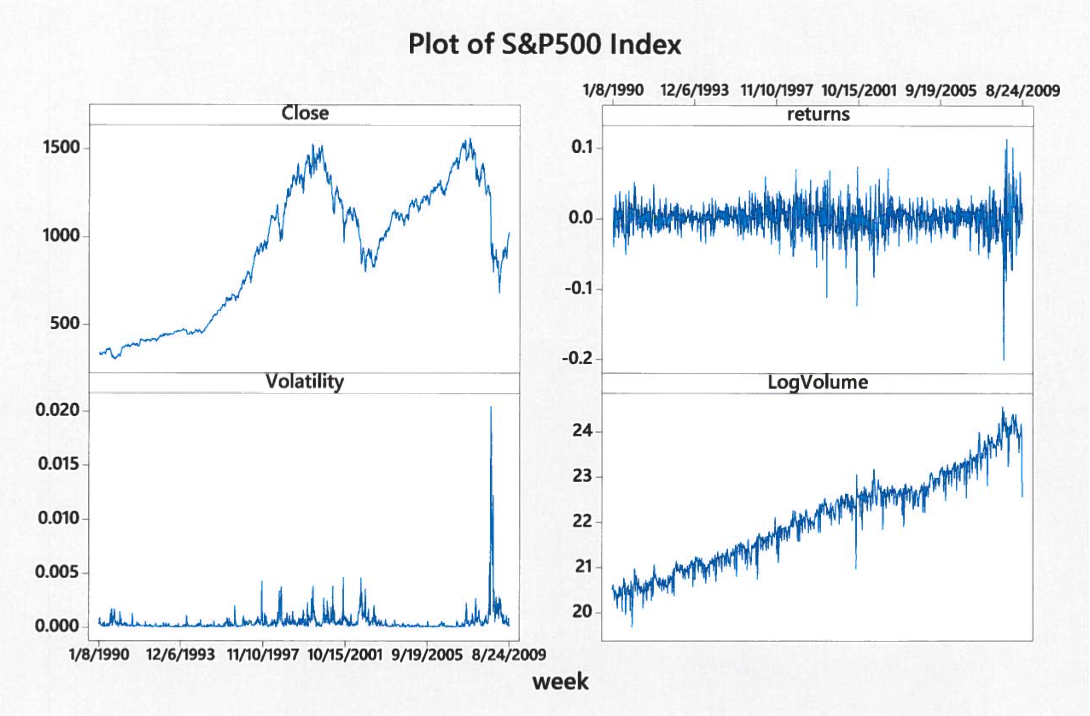
\includegraphics[width=\textwidth]{chapters/chapter_uvts/figures/sp500.png}
	\caption{Plot of S\&P 500 Index. \label{fig:sp500}}
	\end{figure}


In most of the applications of the above regime-switching models, particularly in finance, the plots of relevant quantities clearly reveal the pattern and these models provide a way to confirm the level and size shifts. We want to conclude this section with some simple ideas borrowed from the area of statistical process control. Recall that if the market is efficient, the return $r_t=\ln P_t - \ln P_{t-1}\sim $ IID $(\mu_t, \sigma^2)$, but $\mu_t=\delta$ when $t\geq t_0$ and zero elsewhere. The cumulative sum chart (CUSUM) to detect the positive and negative mean shift are based on recursive calculations:
	\begin{equation}\label{eqn:cdouble}
	\begin{split}
	c_t^+&=\max(0,c_{t-1}^+ + (r_t-k)) \\
	c_t^-&=\min(0,c_{t-1}^- - (r_t-k))
	\end{split}
	\end{equation}
where $k=\delta/2$. The chart signals as sown as $c_t^+$ reaches `$h$'---a decision point set by the user. Jiang, Shu and Apley (2008)~\cite{shuap} modify (\ref{eqn:cdouble}) with exponentially weighted moving average (EWMA) type of estimates that is adaptive in nature. It can be stated as,
	\begin{equation}\label{eqn:elma}
	s_t^+=\max\left(0,s_{t-1}^+ + w(\hat{\delta}_t)\left(r_t - \frac{\hat{\delta}_t}{2}\right)\right)
	\end{equation}
where $w(\hat{\delta}_t)$ is a weight function; a simple weight function $w(\hat{\delta}_t)=\hat{\delta}_t$ is suggested. The $\delta_t$ is updated as 
	\begin{equation}\label{eqn:updatedelt}
	\hat{\delta}_t=(1-\lambda)\, \hat{\delta}_{t-1} + \lambda r_t
	\end{equation}
The adaptive CUSUM chart is effective at detecting a range of mean shift sizes. Similar results for the variance need to be worked out.


In practical applications of these regime-shifting models, it is not easy to discern between a single outlier and persistent level shift. Valid measures that can distinguish these two situations on a timely basis could be very valuable to a trader. We also want to remind the reader that the Markov switching models of changing regimes are indeed latent variable time series models. These models are known as hidden Markov models (HMMs) and represent a special class of dependent mixtures of several processes, these are closely related to state-space models in Section 4.1. An unobservable $m$-state Markov chain determines the state or regime and a state-dependent process of observations. The major difference is that HMMs have discrete states while the Kalman filter based approach refers to unobserved continuous states. 


\section{A Model for Volume-Volatility Relationship}


While the price information via returns and the volatility can be modeled through methods described earlier, it has become important to incorporate other relevant trading data to augment the trading strategies. To that effect, we want to seek some guidance from economic theory how that information is linked to price movements.

In the market microstructure theory, it is assumed that price movements occur primarily due to the arrival of new information and this information is incorporated efficiently into market price. Other variables such as trading volume, bid-ask spread and market liquidity are observed to be related to the volatility of the returns. Early empirical studies have documented a positive relationship between daily trading volume and volatility (See Clark (1973)~\cite{clark}). Epps and Epps (1976)~\cite{epps} and Tauchen and Pitts (1983)~\cite{tauchenpitts} assume that the volume and price are driven by the underlying `latent' information ($I$) and provide a theoretical framework to incorporate this information. Assuming that there are fixed number of traders who trade in a day and the number of daily equilibria, $I$ is random because the number of new pieces of information is random, the return and the volume are written as a bivariate normal mixture model with the same mixing variable $I$. Conditional on $I$:
	\begin{equation}\label{eqn:2rtVt}
	\begin{split}
	 r_t&= \sigma_1\sqrt{I_t}Z_{1t} \\
	 V_t&= \mu_VI_t + \sigma_2\sqrt{I_t}Z_{2t}
	 \end{split}
	 \end{equation}
where $Z_{1t}$ and $Z_{2t}$ are standard normal variables and $Z_{1t}, Z_{2t}$, and $I_t$ are mutually independent. Thus the volatility-volume relationship,
	\begin{equation}\label{eqn:2covVt}
	\begin{split}
	\Cov(r_t^2,V_t)& = E(r_{t}^2V_t) - E(r_t^2) \,E(V_t) \\ 
	&= \sigma_1^2\mu_V \Var(I_t) > 0
	\end{split}
	\end{equation}
is positive due to the variance in $I_t$. If there is no new information or if there is no variation in the mixing variable, $\Var(I_t)= 0$ and thus the relationship vanishes. The theory of arrival rates suggest a
Poisson distribution and based on empirical evidence, the lognormal distribution is taken to be a candidate for distribution of mixing variable, $I_t$. The parameters of the model in (\ref{eqn:2rtVt}) are estimated through maximum likelihood. Gallant, Rossi and Tauchen (1992)~\cite{grt} using a semi-parametric estimate of the joint density of $r_t$ and $V_t$ conduct a comprehensive study of NYSE data from 1925 to 1987. The following summarizes their findings: \\


\noindent\textbf{Stylized Facts 5 (Volume--Volatility Relationship):} 

\begin{itemize}
\item  Positive correlation between conditional volatility and volume.

\item Large price movements are followed by high volume.

\item Conditioning on lagged volume substantially attenuates the leverage (which is an asymmetry in the conditional variance of current price change against past price change) effect.

\item After conditioning on lagged value, there is a positive risk-return relation.
\end{itemize}

These findings can be easily confirmed using the S\&P 500 data presented in Figure~\ref{fig:sp500}. During the period of regime changes (for example, October 1999--November 2000) , we should expect higher volatility and therefore higher correlation with volume. 


Andersen (1996)~\cite{andersen} modifies the model (\ref{eqn:2rtVt}) by integrating the microstructure
setting of Glosten and Milgrom (1985)~\cite{glostenmilgrom} with the stochastic volatility, that is built on weaker conditions on the information arrival process. While the first equation in (\ref{eqn:2rtVt}) remains the same, the volume $V_t$ has informed and noise components, $V_t = IV_t + NV_t$. Noise trading component, $NV_t$ is taken as a time homogeneous Poisson process, $P_0(m_0)$. Therefore, the systematic variation in trading is mainly due to informed volume. Then $IV_t|I_t \sim \text{Poisson}(I_t\mu)$ and thus
	\begin{equation}\label{eqn:2VtIt}
	V_t|I_t \sim \text{Poisson}(m_0 + I_t m_1)
	\end{equation}
It is easy to see $\Cov(r_t^2,V_t) = \sigma^2m_1 \Var(I_t) > 0$ under this setting as well. These models clearly indicate that the intraday return volatility and volume processes jointly contain predictable elements.


There are other studies that focus on the trading volume and returns relationship and we mention only a select few here. Campbell, Grossman, and Wang (1993)~\cite{campbellgross} demonstrate for individual large stocks and stock indices the first-order daily auto-correlation in the returns tend to decline with volume. The authors develop a theoretical model where the economy has two assets, risk-free asset and a stock and there are two types of investors, one with constant risk aversion and the other with risk aversion changing over time. Under this set-up, it is implied that a decline in a stock price on a high-volume day is more likely than a decline on a low-volume day to be associated with an increase in the expected stock return.


Gervais, Kaniel, and Mingelgrin (2001)~\cite{gervais2001high} investigate the role of trading activity in providing information about future prices. It is shown that periods of extremely high (low) volume tend to be followed by positive (negative) excess returns. The formation period for identifying extreme trading volume is a day or a week, but the effect lasts at least twenty days and holds across all stock sizes. To test if this information can be used profitably, the authors construct a trading strategy, by sending buy (sell) limit orders at the existing bid (ask) price, at the end of the formation period. If the orders are not taken, they are converted into market orders at the closing. The strategy is shown to result in profits, in particular with the small-medium firm stocks, after adjusting for the transaction costs. The model used for the empirical framework is the vector autoregressive model discussed later, with an addition of a set of exogenous control variables:
	\begin{equation}\label{eqn:2Ytphi}
Y_t = \Phi_0+\sum_{j=1}^p\Phi_jY_{t-j}+\sum_{l=1}^LB_lX_{t-l}+\epsilon_t
	\end{equation}


The components of $Y_t$ include stock or market related variables such as detrended log of stock turnover, the stock return and the value weighted market return. The control variables are market volatility based on the daily return standard deviation and the dispersion which is the cross-sectional standard deviation of the security returns. The impulse response functions are used to aggregate the overall relationship among the endogenous variables. Statman, Thorley, and Vorkink (2006)~\cite{statman2006investor} show that the trading volume is dependent on past returns over many months and it is argued that this may be due to the overconfidence of the investors.


These and other studies generally confirm the information content of the volume and turnover of stocks traded; strategies to exploit these, especially in a high frequency context, will be examined in Chapter 3. We will discuss how intra-day flow of volume can be related to price changes. 


In algorithmic trading a key ingredient of many strategies is forecast of intra-day volume. Typically a parent order is split into several child orders and the timing of the submission of child orders could depend on the volume forecast for an interval of time that is considered for trading. Brownless, Cipollini and Gallo (2011)~\cite{brownless} provide prediction model for intra-day volume. This will be described in detail in the next chapter.


The model in (\ref{eqn:2rtVt}) is extended to cover multiple stocks in He and Velu (2014)~\cite{hevelu}. The role of common cross-equity variation in trade related variables is of interest in financial economics. The factors that influence the prices, order flows and liquidity are most likely to be common among equities that are exposed to some risk factors. Exploring commonality is useful for institutional trading such as portfolio rebalancing. The mixture distribution in (\ref{eqn:2rtVt}) is developed by assuming that factor structures for returns and trading volume stem from the same valuation fundamentals and depend on a common latent information flow.  


\section{Models for Point Processes}


In many fields of study, observations occur in a continuum, space or time in the form of point events. The continuum can be multi-dimensional, but our focus is on the one-dimensional time scale with points distributed irregularly along the time scale. The main interest lies in estimating the mean rate of occurrence of events or more broadly on the patterns of occurrence. There are excellent monographs on this topic: Cox and Lewis (1966) \cite{cox1966}, Daley and Vere-Jones (2003)~\cite{daley2003}, etc. But the interest in financial applications was revived by the seminal paper by Engle and Russell (1998)~\cite{engle1998}. Financial market microstructure theories as discussed in Kyle (1985) \cite{kyle1985}, Admati and Pfleiderer (1988)~\cite{admati1988theory} and Easley and O' Hara (1992)~\cite{easley1992} suggest that the frequency and the timing of transactions, that include posting, canceling and executing an order, carry information about the state of the market. The transactions generally tend to cluster during certain times of the day and the change in the mean rate of occurrences may suggest a new information flow about a stock.


To illustrate, recall Figure~\ref{fig:tradeactline}, on trading activities in Section 2.1. If we denote the observed intervals between successive activities as durations by $d_1, d_2,\ldots,d_r$, the time of occurrences are obtained by forming the cumulative sums of the $d$'s, $t_1=d_1, t_2=t_1+d_2, \ldots, t_r=t_{r-1}+d_r$. Cox and Lewis (1966)~\cite{cox1966} suggest two ways to present this type of data graphically. One method is based on cumulative numbers of events that have occurred at or before `$t$' against `$t$'. The slope of the line between any two points is the average number of events per unit for that period. One way to standardize the plot would be to approximate the graph by a line, `$at$' when `$a$' is the slope of the graph indicating the average rate of occurrence for the entire duration. The second method calls for dividing the time scale into equally spaced time intervals and count the number of events in each interval; this also can be modified by fixing a certain number of events and spacing on the time it takes for this number to occur. In the context of stock price data, this could mean simply recording not when the trade occurs but when the price changes. The advantage of the second plot is that the local fluctuations are readily observed and the advantage of the first plot is that it enables us to see systematic changes in the rate of occurrence.
 
 	\begin{figure}[!ht]
	\centering	
	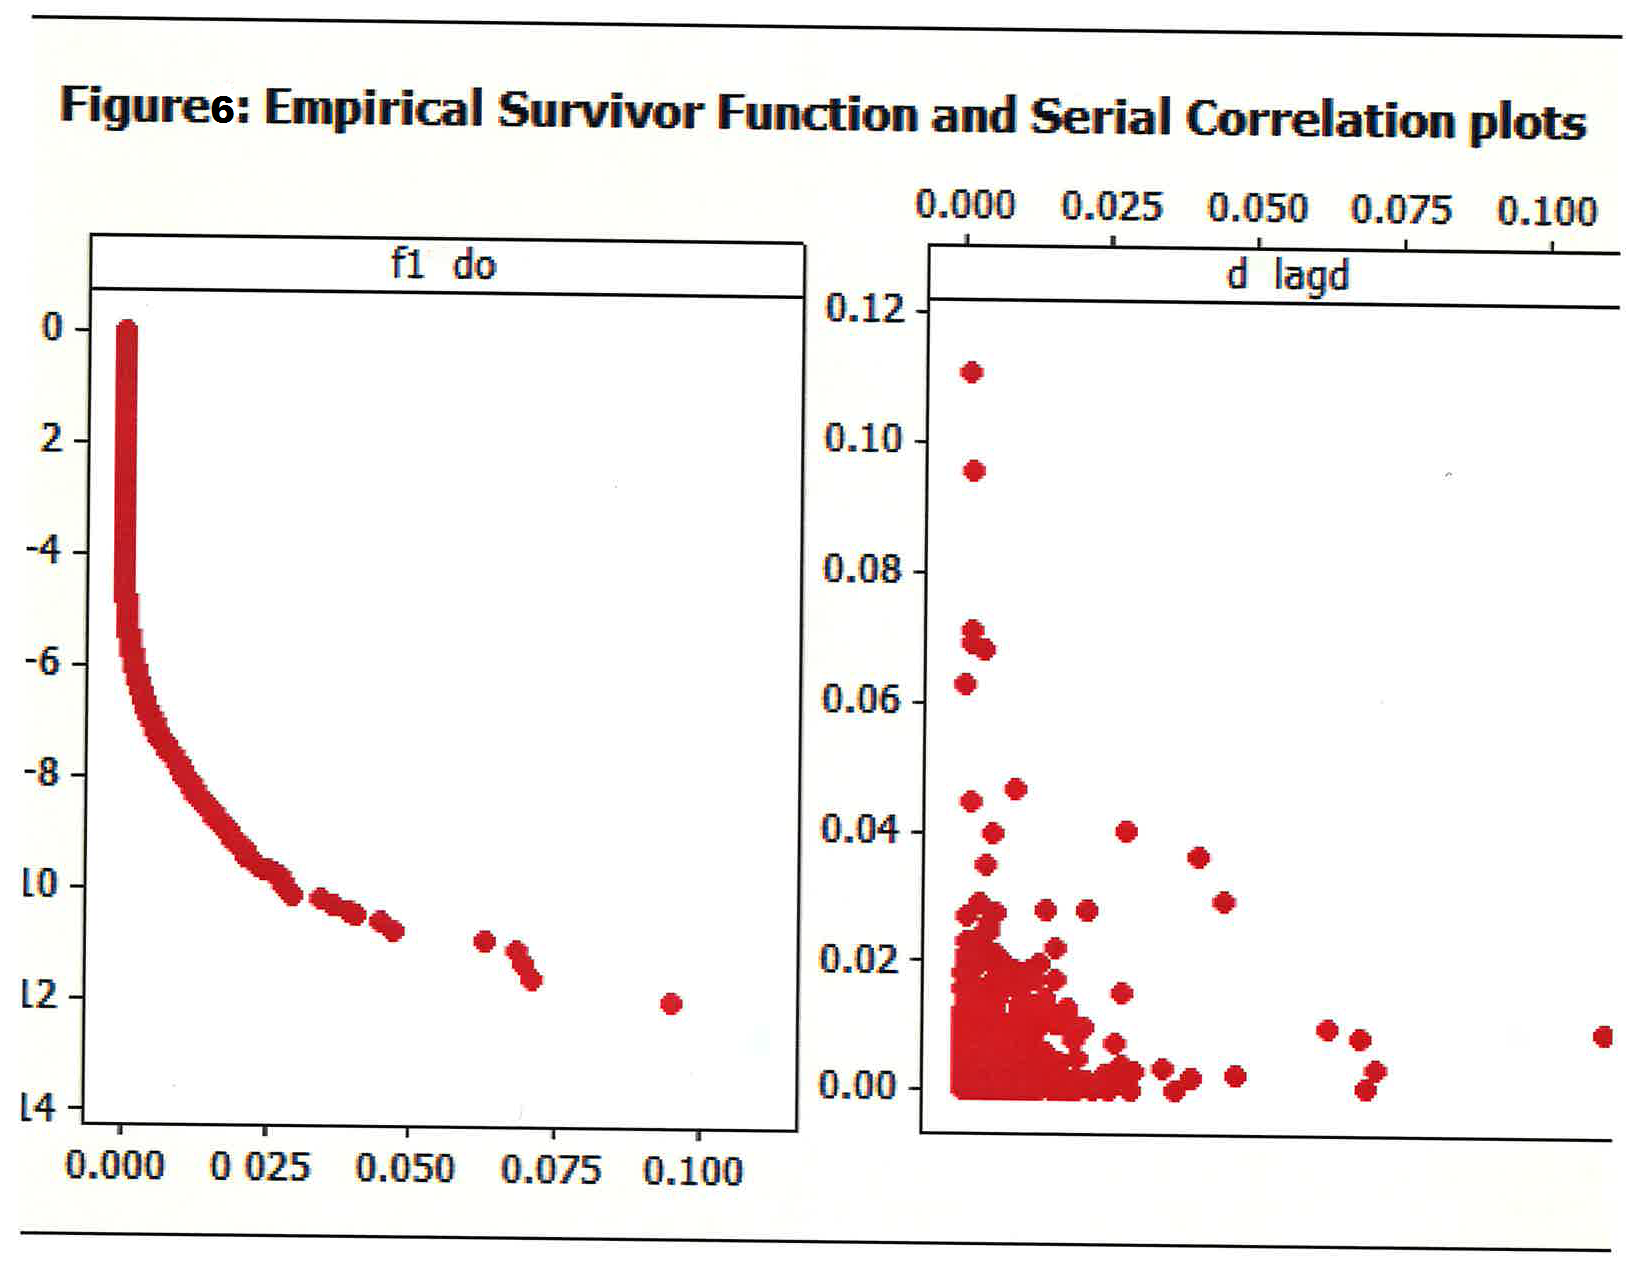
\includegraphics[width=\textwidth]{chapters/chapter_uvts/figures/Sec2-10Fig6.png}
	\caption{Empirical Survivor Function and Serial Correlation plots. \label{fig:survivor}}
	\end{figure}
	
	\begin{figure}[!ht]
	\centering
	 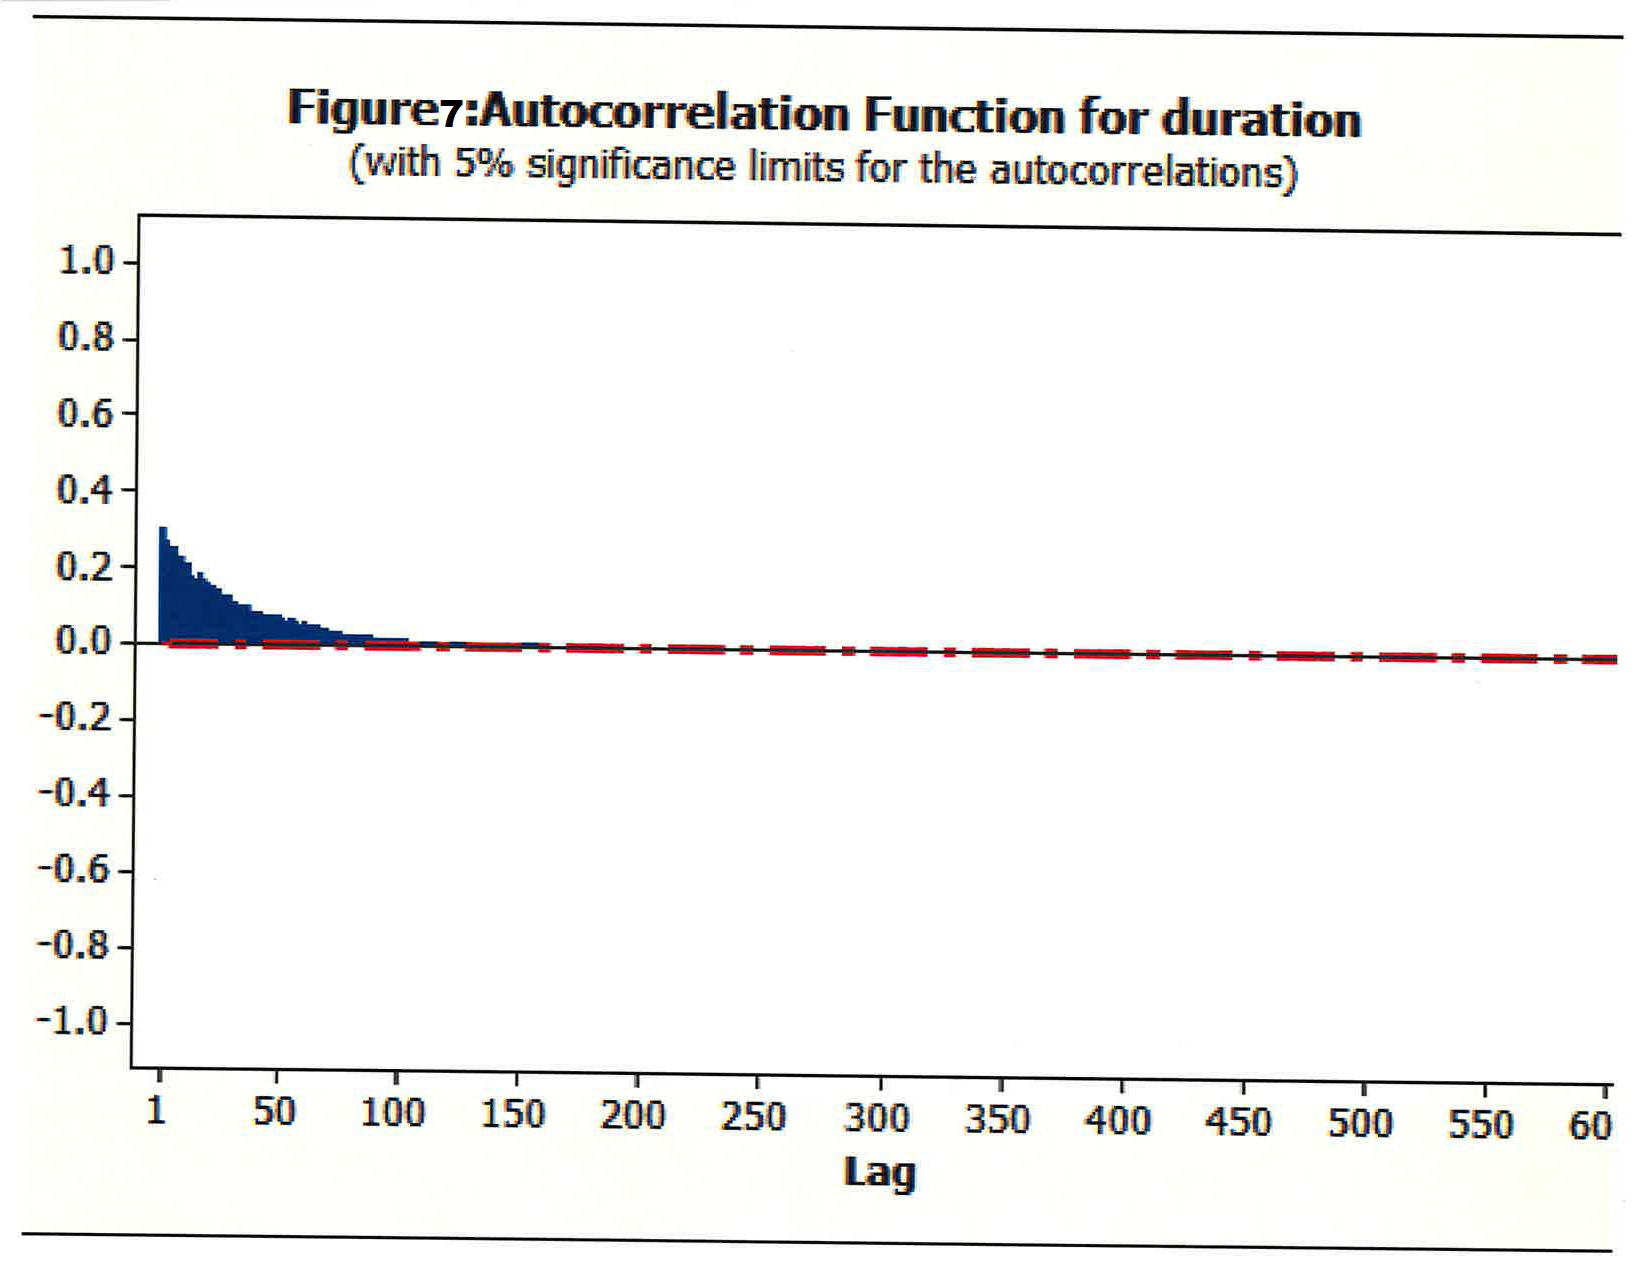
\includegraphics[width=\textwidth]{chapters/chapter_uvts/figures/Sec2-10Fig7.png}
	\caption{Autocorrelation Function for duration. \label{fig:duration}}
	\end{figure}
 
 The baseline distribution for the durations is exponential resulting from Poisson arrivals for a specified interval that assume a constant rate. It is suggested to plot log(1-$\frac{i}{n_0+1})$ against $d_{(i)}$ where $d_{(i)}$ results from the ordered durations, $d_{(1)} \leq d_{(2)} \leq ... \leq d_{(n_0)}$ calculated between successive $n_0+1$ occurrences. Departures from linearity would indicate that the exponential distribution may not hold. In addition it is also suggested to plot $d_{i+1}$ against $d_i$ to check on the dependance of durations. Cox and Lewis (1966, p14)~\cite{cox1966} state that, ``It is not clear how correlation in such data should be measured and tested; in particular it is not obvious that the ordinary correlation coefficient will be the most suitable measure with such data''. Engle and Russell (1998)~\cite{engle1998} show how the dependence in the duration data can be explicitly modeled in the context of high frequency transaction data. We illustrate this with the trading data for Microsoft (MSFT) for the month of January in the year 2013. This graph (Figure~\ref{fig:survivor}) clearly indicates that the durations do not follow an exponential distribution and do exhibit some dependence. This is confirmed by the autocorrelation function for durations (Figure~\ref{fig:duration}).


Cox and Lewis (1966)~\cite{cox1966} also observe a few issues that can arise with the point-process type data. It is possible that two or more events recorded as happening at the same time. This may be due to latency issues but if they occur due to genuine coincidences it is better to analyze the number of events attached to each occurrence time as a variate separately. Further complications are that there may be events, such as price and volume that may be interdependent and events that occur with related series that may be useful for modeling and predicting the future occurrence times.


\subsection{Stylized Models for High Frequency Financial Data}


There has been a great deal of interest in studying market micro-structure to better understand the trading mechanisms and the process of price formation. With the availability of Trades and Quotes (TAQ) data that contains all equity transactions on major exchanges, it has now became possible to better understand the market micro-structure. The extensive details from the order books over multiple exchanges have provided massive amount of data. Analyzing these data will be taken up in later chapters as well. Here we want to present some unique characteristics of the high frequency data and present most commonly used models in practice. To reiterate, the transactions (trades, quotes, bids, etc) may occur at any point in time (Figure~\ref{fig:exchhours}) during the exchange hours as given below.
	\begin{figure}[!ht]
	\centering
	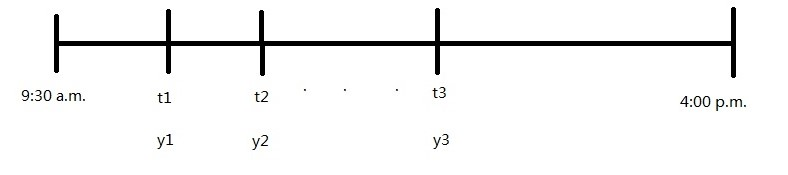
\includegraphics[width=\textwidth]{chapters/chapter_uvts/figures/33d1.jpg}
	\caption{Exchange hours. \label{fig:exchhours}}
	\end{figure}
High-frequency data refer to the `tick' `$t_i$' data which contains, in addition to the exact time of even occurrence, `$y_i$' called marks that may refer to all other elements of the limit order book such as traded price or quote etc. The traditional time series methods that we discussed in the context of low frequency data analysis are not applicable here as the ticks can occur at any point in time when the exchange are open. Standard econometric techniques are for data in discrete time intervals. Aggregating the high-frequency data to some fixed time interval will not capture the advantages of having access to detailed transaction data. Even for some heavily traded stocks, if the intervals are chosen to be short, there may be many intervals with no data and if the intervals are long, the microstructure features will be lost. Also certain key features such as the imbalance between bid side and ask side of the limit order book and when and how the market orders cross the spread are not easy to aggregate in a fixed time interval, however short or long it may be. Moreover, the timings of transactions provide valuable information for trading. Some noted features of high frequency data are:

\begin{itemize}
\item \textbf{Nonsynchronicity:} Different stocks have different trade intensities and even for a single stock, the intensity can vary over a day. For the aggregated low frequency (daily) data, thus, we cannot assume that daily returns occur in equally-spaced time series.

\item \textbf{Multiple transactions with the same time stamp:} It is possible that in periods of heavy trading especially in the opening and closing times of the exchange, each tick may contains multiple transactions. For the analysis of this type of occurrence, simple aggregate summary measures to more elaborate measures such as the variation in prices in addition to average prices are suggested.

\item \textbf{Multiple Exchanges:} In the US market there are at least sixteen known lit exchanges; due to latency issues there could be time delays in recording the submission times of orders that get dispatched at the same time. Also with the rule (NBBO) on getting best price anywhere in the market, an aggregated view of the market given a fixed time interval can miss capturing the dependency over exchanges. 

\item \textbf{Intra-day Periodicity:} Generally, it is observed for stocks transaction activities are higher near the open and the close than in the middle of the data. Thus volatility is higher, immediately after the opening and before the closing of the market resulting in U-shape pattern.

\item \textbf{Temporal Dependence:} High frequency data generally exhibit some dependence. The dependence is due to
    \begin{itemize}
    \item price discoveries
    \item bid-ask bounce
    \item Execution clustering of orders
    \end{itemize}
Under aggregation with low frequency data generally the dependence tends to decrease.

	\begin{figure}[!ht]
	\centering
	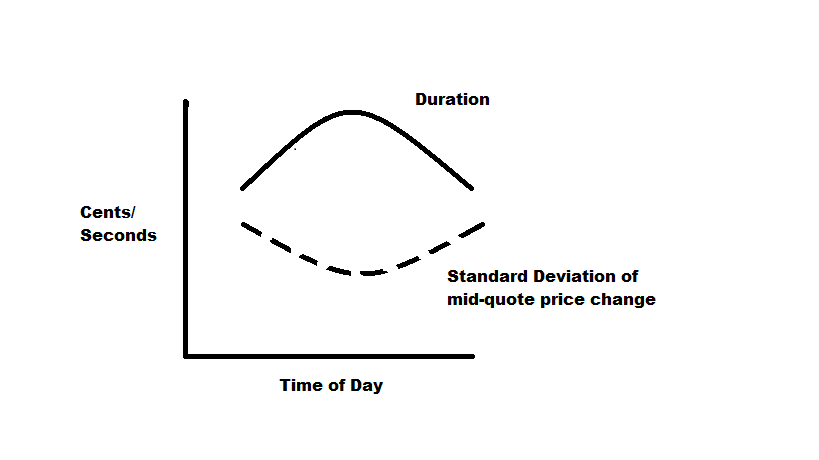
\includegraphics[width=\textwidth]{chapters/chapter_uvts/figures/Sec2-10Fig8.png}	
	\caption{Typical Diurnal patterns. \label{fig:diurnal}}
	\end{figure}

\item Volatility, volume, spread are higher near the open and close.

\item Time between trades, shorter near open and close.
\end{itemize}


\noindent\textbf{Stylized fact 6: Negative autocorrelation in returns:} Non-synchronous trading and bid-ask bounce both can introduce negative lag-1 autocorrelation in the returns. See Roll (1984)~\cite{roll1984} and Lo and Mackinlay (1990)~\cite{lo1990}.


We want to briefly discuss the Roll model; on a typical day of trading stocks exhibit price changes numerous times. These changes signify merely the market friction, the friction between the demand and supply side and they are not necessarily due to true information about the stock. Assume that the true price (unobservable) follows a random walk model, Example~\ref{ex:driftwalk} Chapter 2, as
	\begin{equation}\label{eqn:2plowstar}
	p_t^*=p_{t-1}^* + \epsilon_t 
	\end{equation}
and the observed price,
	\begin{equation}\label{eqn:2lowpstar}
	p_t = p_t^* + u_t
	\end{equation}
with `$\epsilon_t$' denoting the true information about the stock and `$u_t$' denoting the market friction. But the observed return,
	\begin{equation}\label{eqn:2firstrtlow}
	r_t=p_t-p_{t-1} = \epsilon_t + u_t - u_{t-1}
	\end{equation}
inducing the negative autocorrelation of lag 1 in the return due to the carry over term, `$u_{t-1}$'. The term on the right-hand side because of zero autocorrelation beyond lag-1 can be written as MA(1) model:
	\begin{equation}\label{eqn:2lowrt}
	r_t=a_t - \theta a_{t-1}
	\end{equation}
The value of `$\theta$' generally tends to be small, but nevertheless significant. 


\noindent \textit{Commonly used duration models:} The timing aspect of transaction was discussed in Easley and O'Hara (1992)~\cite{easley1992} and a rigorous set of tools was developed by Engle and Russell (1998)~\cite{engle1998}, as an alternative to fixed interval analysis. Treating the ticks as random variables that follow a point process, the intensity of transactions in an interval of length, $\Delta$, is defined as
	\begin{equation}\label{eqn:2lambda}
	\lambda(t) = \lim\limits_{\Delta \rightarrow 0}\frac{E[N(t+\Delta) - N(t)|F_t]}{\Delta}
	\end{equation}
where $N(t)$ denotes the number of ticks until `t' and $F_t$ is the information available until that time. The commonly used model for such arrival rates is Poisson that implies that the time between the two successive ticks is independent of pairwise ticks and follows an exponential distribution. But the duration data, $d_i = t_i - t_{i-1}$ exhibit some dependence, thus implying that time moves faster sometimes, faster than the clock time. The intensity rate, $\lambda(t)$ is not a constant, which is a typical characteristic of the exponential distribution. We briefly outline how the durations are modeled. For detailed discussion, see Tsay (2010)~\cite{tsay} or Lai and Xing (2008, Section 11.2)~\cite{lai1}. The autoregressive conditional duration (ACD) model is defined as follows:
	\begin{equation}\label{eqn:2dipsi}
	\begin{split}
	d_i&= t_i - t_{i-1} = \psi_i\varepsilon_i, \text{ and} \\
	\psi_i&= \alpha + \sum_{j=1}^p\alpha_j d_{t-j} + \sum_{v=1}^q\beta_v\psi_{i-v}
	\end{split}
	\end{equation}
where $\varepsilon_i$ are i.i.d. with $E(\varepsilon_i) = 1$; If $\varepsilon_t's$ are assumed to follow exponential the models (\ref{eqn:2dipsi}) is called E(xpotential)ACD. Two alternative models WACD and GGACD are based on the following specification for the errors:
	\[
	\begin{split}
	\text{Weibull: }h(x) &= \frac{\alpha}{\beta^{\alpha}}x^{\alpha-1}\exp\left\{-(\frac{x}{\beta})^{\alpha}\right\} \\
	\text{Generalized Gamma: } y &= \lambda\frac{x}{\beta}
	\end{split}
	\]
where $\lambda = \frac{\sqrt{K}}{\sqrt{K+\frac{1}{\alpha}}}$. The hazard function of Generalized Gamma is quite flexible and may fit better various patterns. The stationary conditions would require that the roots of $\alpha(B) = 1 - \sum_{j=1}^q(\alpha_j+\beta_j)B^j$ are outside the unit circle when $g= \max(p,q)$ and $B$ is the back-shift operator. It is clear that the model (\ref{eqn:2dipsi}) is similar to GARCH model given in (\ref{eqn:2secondht}). The estimation is typically done through conditional maximum likelihood and all inferences are asymptotic.


An alternative more direct ARMA type model for log durations is suggested by Ghysels, Gourieroux and Jasiak (2004)~\cite{jasiak}:
\begin{equation}\label{eqn:21lnd}
	\ln{(d_i)} = \omega + \sum_{j=1}^p\alpha_j\ln{(d_{t-j})} + \sum_{j=1}^v\beta_j\varepsilon_{i-j} + \varepsilon_i
	\end{equation}
and $\varepsilon_i = \sqrt{h_i^v}u_i, h_i^v = \omega^v + \sum_{j=1}^{p^v}\alpha_j^v\varepsilon_{i-j}^2 + \sum_{j=1}^{q^v}\beta_j^vh_{i-j}^v$ where $u_i \sim N(0,1)$ i.i.d.; here the conditional mean and variance of durations are assumed to be separable. The duration volatility that is modeled using the second equation in (\ref{eqn:2dipsi}) is interpreted as `liquidity' risk. \\


\noindent \textbf{Other Duration Related Models:} So far the discussion has been around modeling the durations, but the information set, $F_t$ has information on `marks', the information associated with the past ticks, such as the number of units transacted, price etc. McCulloch and Tsay (2009)~\cite{} suggest the following model:
	\begin{equation}\label{eqn:2lndi}
	\ln{d_i} = \beta_0 + \beta_1\ln{(d_{t-1})} + \beta_2s_{i-1} + \sigma\varepsilon_i
	\end{equation}
where $s_i$ is the size of the $i$th price change measured in ticks; other relevant variables can be easily added to this model.


\subsection{Models for Multiple Assets: High-Frequency Context}


There is a considerable interest in extending the univariate duration models to multiple stocks or to multiple types of arrival processes. Because investment managers generally consider a portfolio of stocks rather than a single one, it is important for them to follow the transaction processes of several stocks simultaneously. Because of non-synchronous trading relating two stocks with different trading intensities on a common time scale is somewhat difficult. Engle and Lunde (2003)~\cite{englelunde} establish the following model for a bivariate point process for trades and quotes:
	\begin{figure}[!ht]
	\centering
	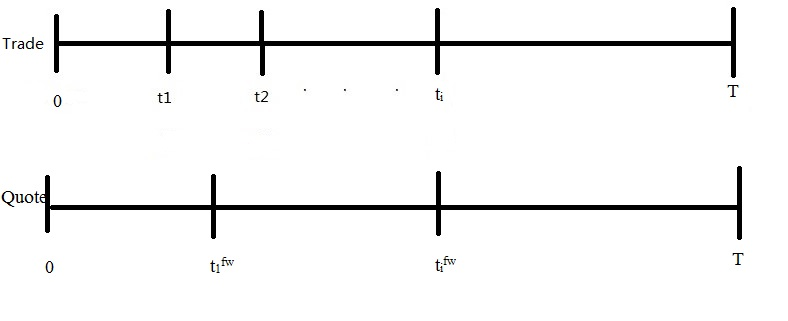
\includegraphics[width=\textwidth]{chapters/chapter_uvts/figures/33d3.jpg}
	\caption{Trades and Quotes. \label{fig:tradeactdoubline}}
	\end{figure}
Define $x_i = t_i - t_{i-1}$ as trade duration and $y_i = t_i^{f_w} - t_{i-1}^{f_w}$ as the forward quote duration; our goal is to model $(x_i,y_i)$ as a bivariate duration process but the underlying timings are not synchronized. Thus define, if $y_i > x_i$, then
	\begin{equation}\label{eqn:anothertildey}
	\widetilde{y}_i = (1 - d_i)y_i + d_ix_i
	\end{equation}
where $d_i$ is indicator variable, $d_i = I_{\{y_i>x_i\}}$. Model ($x_i,\widetilde{y}_i$) as censored process. The equation (98) provides a mechanism in a way to align the two processes. The joint distribution is given by
	\begin{equation}\label{eqn:2pxiyi}
	p(x_i,\widetilde{y}_i | F_{i-1},\omega) = g(x_i|F_{i-1},\omega_1) f(\widetilde{y}_i | x_i,F_{i-1},\omega_2)
	\end{equation}
The first term is the trade density and the second term is the quote density. The $\psi_i$ terms as in (\ref{eqn:}) are modeled as EACD, $\psi_i= f(\psi_{i-1},x_{i-1},z_{i-1})$ and quote density is also modeled as EACD after adjusting for censoring:
	\begin{equation}\label{eqn:2fdot}
	f(y_i|\cdot) = [h(y_i|\cdot)]^{1-d_i} \times S(x_i|\cdot)^{d_i}
	\end{equation}
The estimation of the parameters are done through quasi maximum likelihood. Using data for eight stocks, Engle and Lund (2003)~\cite{englelunde} observe that high trade arrival rates, large volume per trade, wide bid-ask spreads, all predict more rapid price revisions. The model given in Engle and Lund (2003)~\cite{englelunde} can be conceptually applied to any two point processes. Extending this concept to more than two processes could be of interest to the traders who may want to monitor the trading exchanges simultaneously. 



\section{Realized Volatility and Econometric Models}


Estimating the volatility using the high-frequency data has received a great deal of attention lately. In the low frequency (daily) level some estimators based on select prices were presented. Intra-day dynamics of volatility is of interest to traders and that is not fully captured by the stock price indicators sampled during the day. If higher frequency data are used to estimate volatility of lower frequency data, it is important to know the model for the return at the lower frequency. To illustrate this, we consider data observed at two time scales; although they are at low frequency level, the concept can be easily extended to high-frequency context. If $r_{t,i}$ is the $i$th day return in $t$th month, the $t$th month return assuming there `n' trading days, $r_t^m = \sum_{i=1}^nr_{t,i}$. Note that $\sigma_m^2 = \Var(r_t^m|F_{t-1}) = \sum_{i=1}^n \Var(r_{t,i} | F_{t-1}) + 2 \sum_{i<j} \Cov(r_{t-i},r_{t-j} | F_{t-1})$. If $r_{t,i}$ is white noise sequence, then
	\begin{equation}\label{eqn:2hatsigmasq}
	\hat{\sigma}_m^2 = \frac{n}{n-1} \sum_{i=1}^n(r_{t,i} - \overline{r}_t)^2
	\end{equation}
But we had observed that in the high frequency data returns do exhibit some serial correlation and so adjusting (\ref{eqn:2hatsigmasq}) for serial correlation is important to get a more accurate estimate of volatility. A simpler estimate of $\sigma_m^2$ is the so called realized volatility ($RV_t$)
	\begin{equation}\label{eqn:2RV}
	\text{RV}_t = \sum_{i=1}^n r_{t,i}^2
	\end{equation}
But in the estimation of intra-day volatility, the number of sampling intervals, `$n$' and hence, `$\Delta$', the interval size can affect the estimate. If $\Delta \rightarrow 0$, the value $RV_t$ in the $\Delta$-interval goes to infinity. Thus the optimal choice of `$\Delta$' is crucial and is reviewed below, for a judicious choice.


Bandi and Russell (2006)~\cite{bandi} argue that the observed price is the sum of efficient price and a friction price (see (\ref{eqn:2lowpstar})) that is induced by bid-ask bounce, price discreteness etc. Thus the observed variance such as (\ref{eqn:2hatsigmasq}) is the sum of variance of the efficient returns and the variance of micro-structure noise. As they indicate, both are useful: ``The variance of the efficient return process is a crucial ingredient in the practice and theory of asset valuation and risk management. The variance of microstructure noise components reflects the market structure and the price setting behavior of market participants and thereby contains information about the market fine-grain dynamics.'' Both components can be estimated using high frequency data but sampled at different frequencies. Data sampled at low frequency are used to estimate the efficient return variable and the data of high frequency are used to estimate the microstructure noise variance. Additional references on this topic include, A{\"\i}t-Sahalia, Mykland and Zhang (2005)~\cite{ait2005often} and Barndoff-Nielsen and Shepard (2002)~\cite{barndorff2002econometric}.


On any given day, assume that the observed price, at time `$i$' is as in (\ref{eqn:2lowpstar})
	\begin{equation}\label{eqn:2pi2}
	p_i = p_i^* + u_i, \quad i= 1,2,\ldots,n
	\end{equation}
where $p_i^*$ is the efficient price and $u_i$ is the of microstructure noise. Dividing a trading day into $M$ sub-periods, where $\delta= 1/M$ is the size of the sub-period, write the observed returns as
	\begin{equation}\label{eqn:2rji2}
	r_{j,i} = r_{j,i}^* + \varepsilon_{j,i}, \quad j= 1,2,\ldots,M
	\end{equation}
Assume that the frictions, $u$'s are i.i.d. mean zero and variance $\sigma_{u}^2$. Because $\varepsilon_{j,i}= u_{(i-1)+j\delta} - u_{(i-1) + (j-1)\delta}$, $\Var(\varepsilon_{j,i})= 2\sigma_{\eta}^2$. It has been noted already that the return series exhibit negative first order autocovariance and $\varepsilon$'s can be taken as MA(1) structure for the $\eta$'s. Thus, the returns are computed at higher frequency at which the new information arrives. Thus $\sum_{j=1}^M r_{j,i}^2/M$ can be used to estimate noise variance. 


To motivate the optimal choice, we consider two possible situations. If there is no micro-structure noise, the usual estimate of variance, $\hat{\sigma}^2= \frac{1}{T} \sum_{i=1}^n r_i^2$ has the asymptotic variance `$2\sigma^4\delta$' which suggests selecting `$\delta$' as small as possible. The implication of the presence of micro-structure noise is that returns are likely to follow a MA(1) process with a negative autocorrelation and the proportion of total variance due to market micro-structure error is, $\Pi= \frac{2\sigma_\eta^2}{\sigma^2\delta+2\sigma_\eta^2}$ and as `$\delta$' gets smaller, this proportion gets closer to unity. This indicates that the optimal sampling frequency should be finite when noise is present.


For the estimation of efficient price variance, we need to consider an  optimal division of a day into `M' number of subperiods. The optimal sampling frequency over `$n$' day is chosen as $\delta^* = 1/M^*$ with $M^*= \left[\dfrac{\hat{Q}}{\hat{\alpha}}\right]^{\frac{1}{3}}$, where $\hat{\alpha} = \sum_{i=1}^n\sum_{j=1}^M\overline{r}_{j,i}^2/(nM)$ and $\hat{Q}_i = \frac{M}{3}\sum_{j=1}^M\hat{r}_{j,i}^4$. Based on the analysis of a sample of S\&P 100 stocks mid quotes for the months of February 2002, Bandi and Russell (2006)~\cite{bandi} conclude that 5-min frequency is optimal and the 15-min interval may provide the variance estimates `excessively volatile'. The economic benefit of optimal sampling is that high frequency traders can employ a realistic variance forecasts in formulating the entry and exit strategies. 




\section{Analysis of Time Aggregated Data}



The commonly available data from public sources such as Yahoo Finance that are easily accessible to investors provide select price information, High, Low, Open and Close prices along with the total transaction volume in a trading day. The usual estimate of volatility is based on closing prices, but having this additional price (bars) data can help to get a better estimate of volatility. As shown in the last section, using high-frequency data leads to estimators that need to be corrected for market frictions. But using the daily price bars data may not be helpful to make entry/exit decisions; so as a compromise, many trading outfits construct price bars data from the high-frequency point process data for a shorter time intervals such as 30~minutes. This has the effect of smoothing the noise due to market friction but also results in data in discrete time units and so the traditional discrete time series methods discussed in Chapter 2 to Chapter 4 can be effectively employed. 


The price is assumed to follow a random walk model. It follows price changes (thus returns) over a time interval are normally distributed with mean zero and variance that is proportional to the length of the interval. Assuming that the prices follow continuous sample paths although the trading is closed for a certain duration and when trading is open, the actual transactions occur at discrete points in time. Treating the trading day as represented in a unit interval $[0,1]$ with $[0,f]$ representing the `market close' time and $[f,1]$ as `open' time, it is shown that the estimator of volatility
	\begin{equation}\label{eqn:estvol}
	\hat{\sigma}_1^2= \dfrac{(O_1 - C_0)^2}{2f} + \dfrac{(C_1 - O_1)^2}{2(1-f)},
	\end{equation}
has efficiency two compared to the usual estimator, $\hat{\sigma}^2_0=(C_1 - C_0)^2$ based on the closing prices of two successive trading days. This suggests clearly the inclusion of additional data point, opening price is quite informative. Garman and Klass~\cite{klass1980} suggest these and other estimators which are superior to the classical estimator of volatility. It is argued that the high and low prices contain information regarding the volatility during the trading period and a composite estimator
	\begin{equation}\label{eqn:compositeest}
	\hat{\sigma}_2^2= a\,\dfrac{(O_1 - C_0)^2}{f} + (1-a)\, \dfrac{(H_1 - L_1)^2}{(1-f) \ln 2}
	\end{equation}
with optimal choice of `$a$'$=0.17$ that yields even higher efficiency.


The estimators like the above assume that either the price process has no drift or no price jumps between the previous day's closing price and current day's opening price. The former assumption leads to overestimating the volatility and the later to underestimating volatility. Yang and Zhang~\cite{yangzhang2000} provide an estimator based on several periods of low, high, open and close prices that is independent of the drifts and the jumps. Although several estimators are discussed in this paper, we mention only two of them that have high efficiency. Denoting
	\[
	\begin{split}
	o&= \ln O_1 - \ln C_0, \text{ the normalized open}; \\
	u&= \ln H_1 - \ln O_1, \text{ the normalized high}; \\
	d&= \ln L_1 - \ln O_1, \text{ the normalized low}; \\
	c&= \ln C_1 - \ln O_1,  \text{ the normalized close},
	\end{split}
	\]
the classical estimator based on $n$-period historical data is
	\begin{equation}\label{eqn:nperioddata}
	V_{cc}= \dfrac{1}{n-1} \cdot \sum_{i=1}^n [(o_i + c_i) - (\overline{o} + \overline{i})]^2
	\end{equation}
and the estimator given in Rogers and Satchell~\cite{rogerssatchell1991}
	\begin{equation}\label{eqn:rogerssatchell}
	V_{\text{RS}}= \dfrac{1}{n} \cdot \sum_{i=1}^n [u_i(u_i - c_i) + d_i(d_i-c_i)]
	\end{equation}
The estimator suggested in Yang and Zhang~\cite{yangzhang2000} takes the form,
	\begin{equation}\label{eqn:yang2000}
	V_{\text{YZ}}= V_0 + k V_c + (1-k)V_{\text{RS}}
	\end{equation}
where $V_0= \frac{1}{n-1} \sum_{i=1}^n (o_i-\overline{o})^2$ and $V_c=\frac{1}{n-1} \sum_{i=1}^n (c_i - \overline{c})^2$, with the optimal choise of $k=\frac{0.34}{1.34 + (n+1)(n-1)}$. \\


\noindent\textbf{Applications:} It is well-known the standard stochastic volatility models used in finance are difficult to estimate due to their non-Gaussian nature. The proxies, the absolute or squared returns, because of the measurement errors tend to be somewhat inefficient. Alizadeh, Brandt and Diebold (2002)~\cite{diebold} argue that range as a proxy for volatility is superior as it is relatively free of the two problems associated with other measures. In the estimator (\ref{eqn:compositeest}), the second term which is essentially range-based is bound to be always positive. It can also be shown that the standard deviation of the log range is nearly one-fourth the standard deviation of the log absolute return. The range is also more robust to microstructure effects mostly due to bid-ask bounce compared to popular realized volatility measure (\ref{eqn:2RV}). Martens and Dijk (2007)~\cite{dijk} define realized range as,
	\begin{equation}\label{eqn:rrtdelta}
	\text{RR}_t^\Delta= \dfrac{1}{4\ln 2} \cdot \sum_{i=1}^I (\ln H_{t,i} - \ln L_{t,i})^2
	\end{equation}
where `$\Delta$' is intra-day interval. This estimator is biased and the bias is corrected by scaling $\text{RR}_t^\Delta$ with the ratio of average levels of the daily range and the realized range over the previous `$q$' days. The scaled realized range,
	\begin{equation}\label{eqn:rrstdelta}
	\text{RR}_{s,t}^\Delta= \left(\dfrac{\sum_{l=1}^q \text{RR}_{t-l}}{\sum_{l=1}^q \text{RR}_{t-l}^\Delta} \right) \text{RR}_t^\Delta
	\end{equation}
is known to estimate the volatility more accurately. 


The range based statistics can also be used to estimate bid-ask spreads. Recall from (\ref{eqn:2lowpstar}), the Roll model assumes that the observed price is the sum of the true price and the error, that reflects the market friction. The friction can be measured by bid-ask spread which is a measure of market liquidity. Trading decisions are made by closely monitoring this measure that varies during a trading day. Corwin and Schultz (2012)~\cite{schultz12} show how this can be estimated using the low-frequency range-based statistics. The reasoning goes as follows: As noted in (\ref{eqn:2firstrtlow}), the return is the sum of information and the friction---sources of volatility and the bid-ask spread. The volatility increases with the length of the trading period but not the bid-ask spread. Thus the price range over a two-day period reflects two days' volatility and one spread but the sum of two consecutive days price ranges reflect two days' volatility and twice the spread. This reasoning is used to separate the two effects.


Assume that the true or actual price follows a diffusion process. Actual price differs from the true price by $s/2$, where $s$ is the spread that remains constant over two consecutive days. Further, it is assumed that daily high price is a buyer-initiated trade while the daily low price is a seller initiated trade. Write,
	\begin{equation}\label{eqn:sellertrade}
	\begin{split}
	\left[ \ln \left(\dfrac{H_t^0}{L_t^0}\right)\right]^2&= \left[\ln \left(\dfrac{H_t^A(1+s/2)}{L_t^A(1-s/2)}\right)\right]^2 \\
	&=\left[\ln\left(\dfrac{H_t^A}{L_t^A}\right)\right]^2 + 2\alpha \ln\left(\dfrac{H_t^A}{L_t^A}\right) + \alpha^2
	\end{split}
	\end{equation}
where $\alpha=\ln\left(\frac{1+s/2}{1-s/2}\right)$ is taken to be fixed. Taking expectations on both sides, we have
	\begin{equation}\label{eqn:expsides}
	E\left[\ln^2\left(\dfrac{H_t^0}{L_t^0}\right)\right]= K_1\sigma^2 + 2\alpha K_2 \sigma + \alpha^2
	\end{equation}
where $K_1= 4\ln 2= E\left(\ln^2\left(\dfrac{H_t^A}{L_t^A}\right)\right)$ and $K_2=\sqrt{\frac{8}{\pi}}= E\left(\ln\left(\frac{H_t^A}{L_t^A}\right)\right)$. Taking expectations over two days, if we let $\beta=E\left[\sum_{j=0}^1 \ln^2\left(\frac{H_{t+j}^0}{L_{t+j}^0}\right)\right]$ results in 
	\begin{equation}\label{eqn:betaresult}
	\beta= 2K_1 \sigma^2 + 4K_2 \alpha \sigma + \alpha^2
	\end{equation}
which has two unknowns `$\alpha$' and `$\sigma$' to solve. If we let $\gamma=\ln^2\left(\frac{H_{t,t+1}^0}{L_{t,t+1}^0}\right)$, where the subscripts $(t,t+1)$ indicates that the values are computed over a two day period `$t$' and `$t+1$'. This leads to
	\begin{equation}\label{eqn:resultsin}
	\gamma= 2K_1\sigma^2 + 2\sqrt{2} K_2\alpha \sigma + \alpha^2.
	\end{equation}
Both (\ref{eqn:betaresult}) and (\ref{eqn:resultsin}) are two quadratic equations in `$\alpha$' and `$\sigma$' that can be iteratively solved. The explicit solutions are given in Corwin and Schultz (2012)~\cite{schultz12} and are as follows:
	\begin{flalign}\label{eqn:quadsolve}
	&& \sigma&= \dfrac{\sqrt{\dfrac{\beta}{2}} - \sqrt{\beta}}{K_2(3-2\sqrt{2})} + \sqrt{\dfrac{\gamma}{K_2^2(3-2\sqrt{2})}}, && \notag \\ 
	&& \alpha&= \dfrac{\sqrt{2\beta} - \sqrt{\beta}}{3-2\sqrt{2}} - \sqrt{\dfrac{\gamma}{3-2\sqrt{2}}}, && \\
	\text{and} && \phantom{x} & \phantom{x} && \notag \\
	&& s&= \dfrac{2(e^\alpha-1)}{1+e^\alpha}. && \notag
	\end{flalign}
In empirical applications, it has been shown that cross-sectional correlations between the spread estimate in (\ref{eqn:quadsolve}) and TAQ effective spreads (benchmark measure) are higher than any correlations with other estimators. But it has been observed that the above estimator underestimates effective costs for less liquid stocks.


Abdi and Ranaldo (2017)~\cite{abdi} provide an estimator that includes the closing price that is easier to calculate and performs well in terms of the criteria considered earlier. Define the mid-range estimate as, $\eta_t=\frac{\ln H_t + \ln L_t}{2}$ and $c_t=\ln C_t$. Then the effective spread can be obtained from,
	\begin{equation}\label{eqn:obtainedfrom}
	\begin{split}
	s^2&= 4 E\left[\left(c_t - \frac{\eta_t+\eta_{t+1}}{2}\right)^2\right] - E\left[(\eta_{t+1}-\eta_t)^2\right] \\
	&= 4 E\left[(c_t-\eta_t)(c_t-\eta_{t+1})\right]
	\end{split}
	\end{equation}
The sample versions are assuming `$N$' trading days in a month:	
	\begin{flalign}\label{eqn:monthlycorrected}
	&& \hat{s}_{\text{monthly corrected}}&= \sqrt{\max\left\{4 \frac{1}{N} \sum_{t=1}^N (c_t-\eta_t)(c_t-\eta_{t+1}),0\right\}} && \notag \\
	&& \hat{s}_t&= \sqrt{\max\left\{4(c_t-\eta_t)(c_t-\eta_{t+1}),0\right\}}, && \notag \\
	\text{and} && \phantom{x} & \phantom{x} && \\
	&& \hat{s}_{\text{two-day corrected}}&= \dfrac{1}{N}\sum_{t=1}^N \hat{s}_t && \notag
	\end{flalign}
where $\hat{s}_t$ refers to two day estimates. These estimates tend to perform well in terms of both cross-sectional correlates and time series correlations. They also seem to have some predictive power. 



\section{Analytics from Machine Learning Literature}



The technical trading rules that are to be discussed in Chapter 5 involve a relatively small information set to carry out prediction. It treats each of the $n$ time series of asset returns as autonomous. As pointed out by Malkiel (2012)~\cite{malkiel}, these rules can be easily implemented by most market participants if such opportunities should emerge, and market efficiency would rule them out as winning strategies. More powerful prediction methods using a very large set of potential predictors and yet capable of avoiding overfitting are needed to take advantage of transient opportunities. We give a overview here of recent advances in high-dimensional regression and classification and in machine learning and computer science to handle different types of data (including text mining). The literature in this field is vast but we focus only on tools that are deemed to be relevant to trading. 


Machine learning is a growing area of Computer Science that encompasses other well-established areas such as Statistics, computational algorithms, artificial intelligence, Control Theory, etc.. The focus in machine learning is on developing efficient algorithms for prediction using large data sets. The efficiency is gauged by validation accuracy. The inferential aspects of statistical theory, such as standard error of the estimates, confidence intervals, etc., are generally not of much concern. Some areas where machine learning methods have led to significant contribution are classification, clustering and multi-dimensional regression. The attractiveness of these methods lie in the fact that they do not need any a priori theory to suggest relevant variables to consider. Therefore with no prescription of variables, the variable or feature selection becomes an important process in machine learning. The statistical foundations of machine learning methods are generally referred to as statistical learning methods. We provide a brief description of a select few methods in this section. \\

\noindent \textbf{Neural Networks:} The neural network is typically represented as follows:
	\begin{equation}\label{eqn:neural}
	\begin{tikzpicture}[baseline=(current  bounding  box.center)]
	\node(char)[draw,fill=white,shape=rectangle, drop shadow={opacity=.5, xshift=0pt},minimum width=0.7cm, minimum height=0.7cm] at (-4,0) (X) {$\mathbf{X}$};
	\node(char)[draw,fill=white,shape=rounded rectangle, drop shadow={opacity=.5, xshift=0pt},minimum width=0.7cm, minimum height=0.7cm] at (0,0) (Z) {$\mathbf{Z}$};
	\node(char)[draw,fill=white,shape=rectangle, drop shadow={opacity=.5, xshift=0pt},minimum width=0.7cm, minimum height=0.7cm] at (4,0) (Y){$\mathbf{Y}$};
	\draw[->,line width=0.4mm] (X) edge (Z);
	\draw[->,line width=0.4mm] (Z) edge (Y);
	\end{tikzpicture}
	\end{equation}
Here the square boxes contain `$n$' dimensional input or feature vectors, $X$ and `$m$' dimensional output vectors, $Y$ and the circular box indicates hidden or unknown layers in-between that connects the input to the output. From its structure, neural networks are a two-stage regression or classification model with intermediary layers, $Z$ are generally non-linear functions of $X$. In the ordinary least squares regression model, the goal is to get `$m$' linear combinations of `$X$' that best predicts `$Y$'. Here `$r$' dimensional intermediaries can vary based on the assumption of `hidden' layers, but the `key' is that the output vector, `$Y$', can be a non-linear function of `$X$' via the hidden layers. In its simplest form the neural network model can be written as follows:
	\begin{equation}\label{eqn:neurallabel}
	\begin{split}
	z_i&= \sigma(\beta_i'X), \quad i=1,2,\ldots,r \\
	Y_j&= g_j(Z), \quad j=1,2,\ldots,m
	\end{split}
	\end{equation}
where the function $\sigma(u)=\frac{1}{1+e^{-u}}$ is the sigmoid function. Note that this function is used in logistic regression. In the regression set-up, $g_j(Z)=\alpha_j' Z$, but in the $m$-class classification,
	\begin{equation}\label{eqn:gjzclass}
	g_j(Z)= \dfrac{e^{\alpha_j' Z}}{\displaystyle\sum_{l=1}^m e^{\alpha_j' Z}},
	\end{equation}
called the softmax function, is used. In the set-up given in (\ref{eqn:quadsolve}), we assume only one hidden layer, but in practical applications many layers are assumed which leads to non-uniqueness problems. As shown in Hastie, Tibshirani and Friedman (2009)~\cite{hastibf} the neural network problem is closely related to a non-parametric method projection pursuit regression.


To estimate the `$r \times n$' parameters $\beta$'s and `$m \times r$' parameters of $\alpha$'s, the criterion in the regression setting is the usual sum of squares,
	\begin{equation}\label{eqn:bigwtheta}
	W(\theta)= \sum_{l=1}^n \sum_{k=1}^m \big(y_{ik} - f_k(x_i)\big)^2 = \sum_{i=1}^m W_i(\theta)
	\end{equation}
and in the classification setting,
	\begin{equation}\label{eqn:bigwtheta2}
	W(\theta)= - \sum_{i=1}^n \sum_{k=1}^m y_{ik} \ln f_k(x_i),
	\end{equation}
which is a measure of deviance is used. The method to estimate the unknown parameters, `$\theta$' is a gradient descent also called a back-propagation method. This is essentially based on the first differential of $W_i(\theta)$; the `$r \times 1$' iteration is
	\begin{equation}\label{eqn:rby1it}
	\hat{\theta}^{(r+1)}= \hat{\theta}^{(r)} - \gamma_r \sum_{i=1}^n \dfrac{\delta W_i(\theta)}{\delta \theta},
	\end{equation}
where $\gamma_r$ is called the learning rate. Details on the choice of the learning rate are discussed in Hastie et al. (2009)~\cite{hastibf}. Some practical issues in fitting these models are given below. Because these models are over-parametrized, the optimization in (\ref{eqn:rby1it}) can be a nonconvex function.

\begin{enumerate}[--]
\item All inputs need to be standardized as the scaling of these inputs determines the scaling of the weights in the bottom layers.
\item Starting value of `$\theta$' are chosen to be random values near zero as large values tend to result in inferior solutions.
\item Neural Network models tend to overfit the data and so early stopping rates in the iterative process of (\ref{eqn:rby1it}) are suggested. To avoid overfitting, consider minimizing 
	\begin{equation}\label{eqn:overfit}
	W^*(\theta)= W(\theta) + \lambda \theta' \theta,
	\end{equation}
where `$\lambda$' is a positive tuning parameter.
\item Many hidden units ($Z$'s) are preferred as they can capture the non-linearities. 
\item Multiple minima in (\ref{eqn:rby1it}) are possible. A suggested approach to avoid this is `bagging' which are the averages of predictions obtained from random perturbation of training data. 
\end{enumerate}




\section{Exercises}


The dataset consists of (CSV) file that contains the entire trading session, including early and late hours from 6:00~a.m. to 8:00~p.m. EST. It contains intraday depth book activity several major tickers from up to 5 major national exchanges: Nasdaq, Direct Edge, NYSE, ARCA, and BATS (exact number of exchanges depends on the historical period). All messages are consolidates into one file ordered by timestamp. This dataset allows to build a full national depth book (super book) at any moment intraday. 

\begin{table}[h!]
   \caption{Column Format}
   \centering
   \begin{tabular}{p{2cm}p{8cm}} 
   \textbf{Column} & \text{Description} \\ \hline
   Timestamp & Number of milliseconds after the midnight. \\ \hline
   Ticker & Equity symbol (up to 8 characters) \\ \hline
   Order & Unique order ID. \\ \hline
   T & Message type. Allowed Values: \newline
	~~\llap{\textbullet}~~ ``B''--Add buy order \newline
	~~\llap{\textbullet}~~ ``S''--Add sell order \newline
	~~\llap{\textbullet}~~ ``E''--Execute outstanding order in part \newline
	~~\llap{\textbullet}~~ ``F''--Execute outstanding order in full \newline
	~~\llap{\textbullet}~~ ``D''--Delete outstanding order in full \newline 
	~~\llap{\textbullet}~~ ``X''--Bulk volume for the cross event \newline
	~~\llap{\textbullet}~~ ``T''--Execute non-displayed order  \\ \hline
   Shares & Order quantity, available for the ``B'', ``S'', ``E'', ``X'', ``C'', ``T'' messages. Zero for ``F'' and ``D'' messages. \\ \hline
   Price & Order price, available for the ``B'', ``S'', ``X'', and ``T'' order messages. Zero for cancellation and executions. The last 4 digits are decimal digits. The decimal portion is padded on the right with zeros. The decimal point is implied by position; it does not appear inside the price field. Divide by 10000 to convert into currency value. \\ \hline
   MPID & Market Participant ID associated with the transaction (4 characters) \\ \hline
   MCID &U Market Center Code (originating exchange--1 character)
   \end{tabular}
\end{table}


For the analysis of Problems 1--3, we consider the data for CISCO.

\begin{enumerate}[1.]
 
\item You need to aggregate the data into 5-min intervals before answering the following.
\begin{enumerate}[(a)]
\item Let $x_t$ denote the number of trades in the $t$th 5-minute interval. Ignore the time gaps between trading days. Plot the time series and its ACF. Determine if there are intraday period patterns in the series.

\item Using the last transaction in the $t$th 5-minute interval as the stock price in that interval, plot the
time series $y_t$ of 5-minute returns during the period and the corresponding ACF.

\item Consider the bivariate time series ($x_t$, $y_t$). How does $y_t$ vary with $x_t$? Are there intraday periodic patterns in ($x_t$, $y_t$)?

\item Plot the durations of the transaction times for Mondays and Fridays. Is there any difference in the
patterns?

\item Fit GARCH models for the durations and interpret the coefficients.

\item Is there any particular exchange that offers better price?
\end{enumerate}



\item Use the transaction data in Problem 8. There are seventy-eight five-minute intervals in a trading day. Let $d_i$ be the average of all log durations for the $i$th 5-minute interval across all trading days. Let $t_j$ be tick time of a trade during the $i$th 5-minute interval, define an adjusted duration as $\Delta t_j^* = \Delta t_j/\exp(d_i)$ where $\Delta t_j = t_j - t_{j-1}$.
\begin{enumerate}[(a)]
\item Is there a diurnal pattern in the adjusted duration series?

\item Build EACD and WACD models for the adjusted duration and compare them. Now aggregate the data over the 5-minute intervals; Let $r_t$ be the return and $V_t$ is the volume of transactions in the $t$th interval.

\item Is there any relationship between the volume $V_t$ and volatility $r_t^2$ . If there is develop a model that will capture the dependence of volatility on volume. Let $\overline{p}_t$ be the average price in the $t$th 5-minute
interval.
\end{enumerate}


\item Use the CISCO execution data only; aggregate at various time intervals: 1~min, 2~min, \dots, 15~min. For these levels record
\begin{enumerate}[(a)]
\item Average price, VWAP, realized volatility and aggregate volume.

\item By relating the returns and volatility estimates based on average price to realized volatility, identify the optimal duration for aggregation that will cancel out the market friction but pick up the true information. (You may want to refer to Bandi and Russell (2006)~\cite{bandi}). 
\end{enumerate}

\end{enumerate}